\chapter{Étape 6 — Trouver les repères anatomiques}
\label{chap:reperes}

\begin{chapeau}
Cette étape fait le lien entre la segmentation et la planification. Pour chaque fémur et chaque tibia, elle construit
le repère de l'os, reconnaît le côté (droit ou gauche), vérifie que l'os est complet, puis place une vingtaine de
repères anatomiques, mesure les angles articulaires et la torsion. Tout cela prend environ 1,3~s par os.
\end{chapeau}

\section{Orienter l'os}
\label{sec:orienter}

\subsection{L'axe long et le haut de l'os}

L'axe long est la première direction de l'analyse en composantes principales des sommets du maillage
(\cref{sec:acp} et \cref{fig:repere-os}). Il faut ensuite savoir quel bout est proximal :
\begin{itemize}
  \item \textbf{fémur} : le bout qui porte la tête sphérique (celle trouvée à l'étape 3, ou la meilleure sphère ajustée
  à chaque extrémité) ;
  \item \textbf{tibia} : le bout le plus large, le plateau tibial.
\end{itemize}

\fig{repere_os.pdf}{Le tibia du lévrier (a) dans le repère du scanner, avec ses deux premiers axes principaux, et (b)
dans le repère de l'os construit par l'étape 6.}{fig:repere-os}

\subsection{Les côtés anatomiques}

\begin{itemize}
  \item \textbf{Fémur.} Le côté \emph{médial} est celui de la tête (le col part vers l'intérieur). Le côté
  \emph{caudal} est celui de l'échancrure intercondylaire : sur des sections transverses \emph{remplies} juste
  au-dessus du bout distal, c'est le plus grand creux entre la section et son enveloppe convexe.
  \item \textbf{Tibia.} Le côté \emph{crânial} est celui de la crête tibiale : sur des sections du quart proximal, le
  point le plus éloigné du centre. Le côté \emph{latéral} est celui de la fibula ; sans fibula, c'est l'opposé de la
  malléole médiale.
\end{itemize}

\subsection{Droit ou gauche ?}

Avec trois directions anatomiques (latéral $\vb{l}$, proximal $\vb{y}$, caudal $\vb{z}$), le côté découle d'un
produit mixte. Pour un membre droit, le trièdre (latéral, proximal, caudal) est direct :
\begin{equation}
  \text{membre droit} \iff (\vb{l} \times \vb{y}) \cdot \vb{z} > 0.
\end{equation}
Le logiciel compare ce côté « anatomique » au côté lu dans le repère du scanner (en LPS, $+x$ est la gauche du
patient) et prévient s'ils diffèrent : la position du patient a pu être mal déclarée sur la console. Un membre gauche
est ensuite mis en miroir (\cref{eq:repere-os}) et traité comme un droit.

\section{Vérifier que l'os est complet}
\label{sec:completude}

La méthode CORA a besoin des \textbf{deux articulations} de l'os. Un os coupé par le bord du champ du scanner est donc
refusé, avec la raison. Deux méthodes :
\begin{itemize}
  \item si l'étape 4 a noté les bords du champ touchés par l'os : une extrémité est coupée si des sommets de son
  dixième extrême sont à moins de 1,5~mm d'un de ces plans ;
  \item si l'on n'a que le STL : une extrémité coupée porte un « couvercle », une face plane perpendiculaire à un axe du
  scanner. On la détecte à plus de 80~mm² de facettes coplanaires (à 0,3~mm près) dont la normale est à moins de
  2\degre{} de cet axe. Sur le lévrier, les couvercles mesurent 122 et 146~mm², alors qu'aucune surface naturelle ne
  dépasse 47~mm².
\end{itemize}

\section{Le repère de l'os, en trois passes}
\label{sec:repere-construction}

Le repère final est défini par des repères anatomiques, mais ces repères se cherchent plus facilement dans un repère
déjà bien orienté. Le logiciel alterne donc trois fois : repère → repères → nouveau repère.

À chaque passe, on donne une direction $\vb{y}$ (proximale) et une direction approchée $\vb{x}$ (latérale). Le repère
est rendu orthonormé direct par le procédé de Gram--Schmidt :
\begin{equation}
  \vb{e}_Y = \frac{\vb{y}}{\norm{\vb{y}}}, \qquad
  \vb{e}_X = \frac{\vb{x} - (\vb{x}\cdot\vb{e}_Y)\,\vb{e}_Y}{\norm{\vb{x} - (\vb{x}\cdot\vb{e}_Y)\,\vb{e}_Y}}, \qquad
  \vb{e}_Z = \vb{e}_X \times \vb{e}_Y.
\end{equation}

\begin{itemize}
  \item \textbf{Tibia} : $\vb{y}$ = axe mécanique, de l'éminence intercondylaire au centre distal ; $\vb{x}$ = ligne
  des points caudaux des condyles tibiaux, de médial à latéral.
  \item \textbf{Fémur} : $\vb{y}$ = axe anatomique, par les milieux de la diaphyse à 1/3 et à 1/2 de la longueur depuis
  le haut \cite{tomlinson2007} ; $\vb{x}$ = ligne des points caudaux des condyles.
\end{itemize}

L'origine est enfin placée au centre de l'articulation distale, au niveau du bout distal de l'os. C'est une simple
translation : les repères sont décalés, pas recalculés.

\section{Les outils géométriques}

Les repères sont trouvés par quelques outils simples, qui imitent les gestes du chirurgien sur une radiographie.

\textbf{Le point extrême.} Le point le plus proximal du côté latéral (sommet du grand trochanter), le point le plus
crânial (tubérosité tibiale), les points extrêmes en $X$ (épicondyles, malléoles).

\textbf{La tangente commune.} Sur une radiographie de face, le chirurgien pose une règle sous les deux condyles. Le
logiciel fait la même chose avec l'\emph{enveloppe convexe} 2D des points de la zone distale, projetés dans le plan de
la vue : l'arête de l'enveloppe qui relie un point du côté médial et un point du côté latéral, en bas, est la règle
(\cref{fig:tangente}). Elle ne dépend pas de la forme du creux entre les condyles, et une fabelle (toujours plus
proximale) ne peut pas la toucher.

\fig{tangente_commune.pdf}{La tangente commune, trouvée comme une arête de l'enveloppe convexe : sur le fémur du
lévrier (vue de face, zone distale) et en principe. En bleu l'enveloppe convexe, en rouge l'arête qui enjambe le
creux.}{fig:tangente}

\textbf{La sphère.} Le centre de la tête du fémur et ceux des condyles sont des centres de sphères ajustées par RANSAC,
puis par moindres carrés (\cref{eq:sphere}). On n'y garde que les points dont la normale s'éloigne du centre : une
surface convexe vue de l'extérieur.

\textbf{La région articulaire.} Une surface articulaire est trouvée par croissance de région \emph{sur le maillage} :
on part d'un sommet et on ajoute les sommets voisins dont la normale est proche de celle du plateau (moins de 40\degre).

\textbf{La section et son milieu.} Le milieu de la diaphyse à une hauteur $y$ est le milieu des bords médial et latéral
(en $X$) et des bords crânial et caudal (en $Z$) de la coupe de l'os par le plan horizontal, comme on le mesure sur deux
radiographies. Pour voir les creux et les saillies, la coupe est \emph{remplie} ligne par ligne par la règle
pair--impair (on entre dans l'os à chaque croisement impair du contour).

\section{Les repères trouvés}

\begin{table}[htbp]
\centering\small
\caption{Les repères anatomiques et la façon dont le logiciel les trouve.}
\label{tab:reperes}
\begin{tabularx}{\linewidth}{L{4.3cm}Y}
\toprule
\titrecol{Repère} & \titrecol{Méthode} \\
\midrule
\rowcolor{entete!45}\multicolumn{2}{l}{\titrecol{Fémur}} \\
centre de la tête & sphère robuste sur le cinquième proximal \\
sommet du grand trochanter & point le plus proximal du côté latéral \\
centre du col & barycentre de la surface hors de la tête, dans une coquille de 1,1 à 1,6 rayon de tête \\
base du col (petit trochanter) & milieu de la section au niveau de la saillie caudo-médiale maximale \\
points distaux des condyles & tangente commune sous les condyles (vue de face) \\
points caudaux des condyles & tangente commune derrière les condyles (vue axiale), sous le centre des condyles \\
centres des condyles & sphères sur les surfaces distales et caudales \\
épicondyles médial et latéral & points extrêmes en $X$ au niveau des centres des condyles \\
fond de la trochlée & sillon suivi niveau par niveau sur la face crâniale \\
\midrule
\rowcolor{entete!45}\multicolumn{2}{l}{\titrecol{Tibia}} \\
éminence intercondylaire & milieu des sommets des tubercules médial et latéral \\
centres des plateaux médial et latéral & centre de chaque région articulaire (croissance de région sur le maillage) \\
bords crânial et caudal du plateau médial & extrêmes en $Z$ de la région, dans une bande centrale \\
points caudaux des condyles & tangente commune derrière l'extrémité proximale \\
tubérosité tibiale & point le plus crânial de l'extrémité proximale \\
sillons de la cochlée, crête intermédiaire & profil haut de la surface distale : deux pics séparés par un creux \\
bords crânial et caudal de la surface distale & extrêmes en $Z$ près de la crête \\
saillies crâniales distales & tangente commune juste au-dessus de la cochlée (axe antécochléaire) \\
malléoles & points extrêmes en $X$ du bout distal (la latérale est sur la fibula) \\
\bottomrule
\end{tabularx}
\end{table}

\fig{reperes_femur.png}{Les repères trouvés automatiquement sur le fémur du lévrier, vus de face, de profil et du
dessus (fichier \fichier{cora_femur.png}).}{fig:reperes-femur}

\begin{attention}[title={La cochlée vue de face}]
La surface articulaire distale du tibia est creuse d'avant en arrière. Sur une radiographie de face, le rayon X est
tangent à sa partie la plus profonde. Le trait visible est donc l'enveloppe \emph{haute} de la surface : c'est sur ce
profil que le logiciel cherche les deux sillons et la crête, pour mesurer comme sur une radiographie.
\end{attention}

\section{Les angles articulaires}
\label{sec:angles}

Les angles sont mesurés en \textbf{projection}, comme sur une radiographie : de face, on garde $(x, y)$ ; de profil,
$(z, y)$. Pour deux vecteurs projetés $\vb{a}$ et $\vb{b}$, on utilise l'angle non orienté et l'angle orienté :
\begin{equation}
  \angle(\vb{a}, \vb{b}) = \arccos\frac{\vb{a}\cdot\vb{b}}{\norm{\vb{a}}\,\norm{\vb{b}}},
  \qquad
  \measuredangle(\vb{a}, \vb{b}) = \atantwo\bigl(a_1 b_2 - a_2 b_1,\ \vb{a}\cdot\vb{b}\bigr).
\end{equation}
Avec $\vb{d}$ la direction de l'axe vers distal (tibia : de l'éminence au centre distal ; fémur : axe anatomique), et
les indices F (face) et S (profil) pour les projections :
\begin{align}
  \mathrm{mMPTA} &= \angle\bigl(\text{plat}_{\text{méd}} - \text{plat}_{\text{lat}},\ \vb{d}\bigr)_F, &
  \mathrm{mMDTA} &= \angle\bigl(\text{sillon}_{\text{méd}} - \text{sillon}_{\text{lat}},\ -\vb{d}\bigr)_F, \\
  \mathrm{mCaPTA} &= \angle\bigl(\text{plat}_{\text{caud}} - \text{plat}_{\text{cran}},\ \vb{d}\bigr)_S, &
  \mathrm{mCrDTA} &= \angle\bigl(\text{dist}_{\text{cran}} - \text{dist}_{\text{caud}},\ -\vb{d}\bigr)_S, \\
  \mathrm{aLPFA} &= \angle\bigl(\text{trochanter} - \text{tête},\ \vb{d}\bigr)_F, &
  \mathrm{aLDFA} &= \angle\bigl(\text{cond}_{\text{lat}} - \text{cond}_{\text{méd}},\ -\vb{d}\bigr)_F, \\
  \mathrm{aCdDFA} &= \angle\bigl(\text{caud}_{\text{milieu}} - \text{trochlée},\ -\vb{d}\bigr)_S. & &
\end{align}

\fig{angles_reels.pdf}{Les angles articulaires mesurés par le logiciel sur le fémur et le tibia du lévrier (os gauches,
mis en miroir). Tous sont dans les normes (\cref{tab:normales-levrier}).}{fig:angles-reels}

\section{La torsion}
\label{sec:torsion}

La torsion est un angle orienté \emph{autour} de l'axe long $\vb{n}$, entre un axe transverse proximal $\vb{a}$ et un
axe transverse distal $\vb{b}$ (\cref{fig:torsion}). On projette d'abord les deux axes sur le plan perpendiculaire à
$\vb{n}$, puis on mesure l'angle orienté dans ce plan :
\begin{equation}
  \tcbhighmath{\vb{a}_\perp = \vb{a} - (\vb{a}\cdot\vb{n})\,\vb{n}, \qquad
  \vb{b}_\perp = \vb{b} - (\vb{b}\cdot\vb{n})\,\vb{n}, \qquad
  \tau = \atantwo\bigl((\vb{a}_\perp \times \vb{b}_\perp)\cdot\vb{n},\ \vb{a}_\perp\cdot\vb{b}_\perp\bigr).}
  \label{eq:torsion}
\end{equation}

\begin{figure}[htbp]
\centering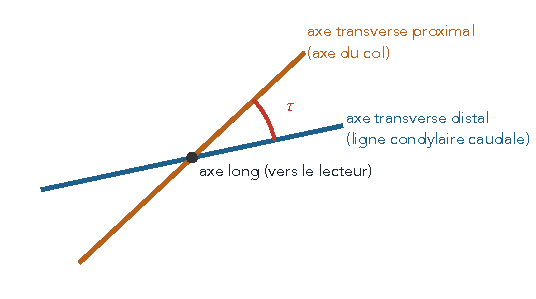
\includegraphics[width=0.5\linewidth]{torsion.pdf}
\caption{La torsion $\tau$ : l'angle, vu le long de l'axe de l'os, entre un axe transverse proximal et un axe transverse
distal.}
\label{fig:torsion}
\end{figure}

Le logiciel utilise les définitions publiées au scanner :
\begin{itemize}
  \item \textbf{fémur} (antéversion, Al Aiyan 2021 \cite{alaiyan2021}) : axe long = axe anatomique ; axe proximal = du
  centre de la tête à la base du col au niveau du petit trochanter ; axe distal = ligne des points caudaux des
  condyles ; $+$ = col dirigé vers crânial ;
  \item \textbf{tibia} (Brühschwein 2023 \cite{bruhschwein2023t}) : axe long par les centres de la diaphyse à 25 et
  75~\% de la longueur ; axe proximal = ligne des points caudaux des condyles ; axe distal = axe antécochléaire ;
  $-$ = interne, $+$ = externe.
\end{itemize}

\begin{exemple}
Lévrier : antéversion de 25,1\degre{} (normale : 20 à 35\degre) et torsion tibiale de $-7{,}9\degre$ (normale : $-10$
à $+2\degre$). Les anciennes définitions du prototype (axe du col au ras de la tête, axe bimalléolaire) donnaient
15,6\degre{} et $+6{,}0\degre$ : deux fausses « torsions externes » sur un chien sain. La définition compte autant que
la mesure.
\end{exemple}

\section{Valeurs normales et écart de définition}
\label{sec:calibration}

Les valeurs normales publiées sont mesurées sur radiographie, avec des repères placés à la main. Nos repères 3D n'ont
pas exactement la même définition. Comparer directement serait faux de plusieurs degrés pour certains angles de
profil, dont les lignes articulaires sont courtes (20 à 30~mm : 1~mm sur un bord arrondi change l'angle de 2 à
3\degre).

Nous mesurons donc l'\textbf{écart de définition} une fois pour toutes, sur l'os sain de l'os fictif, dont les repères
« radiographiques » sont connus :
\begin{gather}
  \Delta = \text{angle}(\text{repères détectés}) - \text{angle}(\text{repères du modèle}), \nonumber \\
  \text{valeur normale utilisée} = \text{valeur publiée} + \Delta.
\end{gather}
Comme les deux mesures sont faites sur le même os, l'écart ne vient que des définitions. Il est faible de face
(aLPFA $+0{,}15\degre$, aLDFA $+0{,}01\degre$, mMPTA $+1{,}30\degre$, mMDTA $+0{,}14\degre$) et plus grand de profil
(aCdDFA $-8{,}2\degre$, mCaPTA $+9{,}5\degre$, mCrDTA $+5{,}1\degre$). Le résultat est gardé en cache dans
\fichier{calibration_reperes.json} et recalculé si le code de l'étape 6 change.

\begin{table}[htbp]
\centering\small
\caption{Les angles du lévrier et les valeurs normales dans la définition du logiciel (moyenne ± écart-type). Un
angle est jugé anormal à plus de deux écarts-types.}
\label{tab:normales-levrier}
\begin{tabular}{llrrr}
\toprule
\titrecol{Os} & \titrecol{Angle} & \titrecol{Lévrier} & \titrecol{Normale} & \titrecol{Écart / écart-type} \\
\midrule
fémur & aLPFA & 114,2\degre & 103,2 ± 6,4\degre & $+1{,}7$ \\
 & aLDFA & 96,3\degre & 94,0 ± 3,3\degre & $+0{,}7$ \\
 & aCdDFA & 88,7\degre & 88,1 ± 6,3\degre & $+0{,}1$ \\
tibia & mMPTA & 91,2\degre & 94,6 ± 1,8\degre & $-1{,}9$ \\
 & mMDTA & 96,5\degre & 96,1 ± 2,7\degre & $+0{,}1$ \\
 & valgus tibial & 7,7\degre & 13,2 ± 3,1\degre & $-1{,}8$ \\
 & mCaPTA & 77,7\degre & 73,2 ± 2,6\degre & $+1{,}7$ \\
 & mCrDTA & 84,5\degre & 86,7 ± 3,2\degre & $-0{,}7$ \\
\bottomrule
\end{tabular}
\end{table}

\section{Choisir l'os à planifier}

Le chirurgien arrive en général avec \textbf{un scanner pour un os}. Le logiciel retient les fémurs et les tibias
complets. S'il y en a plusieurs, il propose le plus éloigné des normes (la somme des écarts en écarts-types). Si le
même os est complet des deux côtés, l'autre devient le \textbf{membre controlatéral}, la meilleure référence. Le choix
et sa raison sont écrits dans \fichier{cora_cas.json} et affichés dans la carte \ui{Os à planifier (CORA)}.

\section{Validation}

\begin{itemize}
  \item \textbf{Os fictif posé au hasard} (4 poses, dont 2 en miroir) : côté reconnu 8 fois sur 8 ; repères à moins de
  0,84~mm des repères exacts au fémur et de 0,98~mm au tibia ; mêmes repères dans les quatre poses (écart nul dans le
  repère de l'os).
  \item \textbf{Lévrier} : les trois os coupés par le champ sont refusés ; les angles du fémur et du tibia complets
  sont dans les normes ; l'os déplacé puis mis en miroir donne les mêmes repères.
\end{itemize}

\begin{danslecode}
\fichier{code_source/etape6_reperes.py} : classe \code{Os} (repère courant, \code{poser()}, \code{section_remplie()},
\code{milieu_diaphyse()}), \code{orienter()}, \code{extremites_coupees()}, \code{analyser()} (les trois passes),
\code{reperes_femur()}, \code{reperes_tibia()}, \code{enveloppe_tangente()}, \code{sphere_robuste()},
\code{region_connexe()}, \code{angles_articulaires()}, \code{torsion()}, \code{calibration()}, \code{normales()},
\code{choisir_cible()}. Sorties : \fichier{cora_<os>.json}, \fichier{cora_<os>.bin} (maillage dans le repère de l'os),
\fichier{cora_<os>.png}, \fichier{cora_cas.json}.
\end{danslecode}
